\documentclass[french,a4paper,12pt]{report}
\usepackage[utf8]{inputenc}
\usepackage[T1]{fontenc}
%\Package paramétrage: marge horizontale à 2,5 cm, et la marge verticale à 1,5 cm.
\usepackage{geometry}
\geometry{hmargin=2.5cm,vmargin=3cm}
\usepackage{eso-pic}
\usepackage{graphicx}
\usepackage{float}
\usepackage{listings}
\usepackage{color}
\definecolor{dkgreen}{rgb}{0,0.6,0}
\definecolor{gray}{rgb}{0.5,0.5,0.5}
\definecolor{mauve}{rgb}{0.58,0,0.82}

\lstset{frame=tb,
  language=Java,
  aboveskip=3mm,
  belowskip=3mm,
  showstringspaces=false,
  columns=flexible,
  basicstyle={\small\ttfamily},
  numbers=none,
  numberstyle=\tiny\color{gray},
  keywordstyle=\color{blue},
  commentstyle=\color{dkgreen},
  stringstyle=\color{mauve},
  breaklines=true,
  breakatwhitespace=true,
  tabsize=3
}

%\hfill\hbox to 0pt{\hss
\includegraphics[width=7cm]{UTBM_LOGO.png}\hss}\hfill\null\newline
\begin{document}



\title{	Université de technologie de Belfort-Montbéliard \\
		{\large \textsc{Informatique, spécialisé dans les systèmes embarqués }} \\
		\vspace{1cm}
		Contrôle Haptique et Asservissement de la Mécanique des Pianos de concert
	  }
	  
\date{5 Février 2018 -- 13 Juillet 2018 }
	  
\author{Professeur suiveur : GECHTER Franck  \\
		Tuteur de stage		: LEBBOLO Hervé  \\
		Elève				: ROMET Pierre
		}

\makeatletter
  \begin{titlepage}
  \centering
  \
      {\large \textsc{ }}\\
      \textsc{}\\
      
      \vfill
       {\LARGE \textbf{\@title}} \\
    	\vspace{2em}     
      
    \vspace{1cm}
      {\large{	\@date\\
    \vspace{1cm}
       Stage ST50}}\\
    \vspace{1cm}
        {\large \@author} \\
    \vfill
        
\includegraphics[height=0.13\textheight]{UTBM_LOGO.png}
        \hfill
        
\includegraphics[height=0.09\textheight]{LPNHE_LOGO.png}
  \end{titlepage}
\makeatother

\tableofcontents

\part{Préambule}

  \chapter{Remerciement}
  Tout d'abord je tiens à remercier l'ensemble de mes collègues pour l'accueille des plus chaleureux, au sein du laboratoire de physique nucléaire et des hautes énergies, ainsi que pour leur présence tout au long de mon stage, en m'aidant et me conseillant.\newline
  
  Je voudrais remercier Monsieur Olivier LEDORTZ pour son aide concernant le langage VHDL.\newline
  
  Je tiens à remercier mon maitre de stage Monsieur Hervé LEBBOLO, pour son implication dans l'encadrement de mon stage, son soutien, ainsi que pour l'ensemble des connaissances transmises dans le domaine de l'électronique analogique.\newline
  
  Enfin, je tiens également à remercier mon enseignant suiveur, Monsieur Franck GECHTER, grâce à qui j'ai pu réaliser un stage de fin d'étude me permettant d'allier mon corps de métier, à une passion, la musique.
  
 \chapter{Introduction}

Dans le cadre des mes études d'ingénieurs au sein de l'Université de Technologie de Belfort-Montbéliard, j'ai effectué un stage de fin d'étude en laboratoire d'une durée de 24 semaines au sein du Laboratoire de Physique Nucléaire et des Hautes Énergies à Paris.\newline

Le laboratoire de Physique Nucléaire et des Hautes Énergies est une unité de recherche de l'institut national de  physique nucléaire et de physique des particules, institut du CNRS et des universités Sorbonne Université et Paris Diderot.\newline

Mon stage s'est déroulé au sein du service électronique, sous la tutelle de Monsieur Hervé LEBBOLO.\newline

Lors de ce stage, je fut recruté pour travailler sur le projet "CHAMP"; projet initié par Antoine "NOMDEFAMILLE", afin de mettre en place un contrôle haptique, ainsi qu'un asservissement, de la mécanique de Pianos de concert.\newline

Le laboratoire étant spécialisé dans le domaine de l'électronique embarqué, travaillant par exemple, sur un nouveaux télescope spatial, ce stage fut pour moi l'occasion d'évoluer dans un domaine des systèmes embarqués que je ne maitrisais peu, (de part ma formation) l'électronique analogique et numérique, ce qui m'as permis de découvrir et d'acquérir de nouvelles compétences ainsi que les méthodes de développement qui y sont lié.\newline

Suite à cette introduction, nous allons poursuivre avec la présentation du laboratoire (LPNHE), puis nous conclurons cette premières partie par la présentation du projet "CHAMP".


  
  \chapter{Présentation du laboratoire}
  Le LPNHE a été fondé par un groupe de chercheurs et enseignants-chercheurs issus de la division « hautes énergies » de l’institut de Physique Nucléaire (IPN) d’Orsay. En 1970, ces spécialistes des chambres à bulles rejoignent l’université Paris VI et l’ensemble devient un laboratoire associé au CNRS. A cette époque, la recherche s’y organise principalement autour d’expériences de chambres à bulles au CERN. Le LPNHE a donc derrière lui une longue histoire de collaboration avec le CERN. 
  
  Aujourd’hui encore, même si les expériences et projets dans lesquels est engagé le laboratoire se trouvent maintenant sur les cinq continents, le CERN reste l’endroit privilégié où les chercheurs de physique des particules du laboratoire effectuent leur recherche.
  
  Le Laboratoire de Physique Nucléaire et des Hautes Énergies est une unité de recherche de l'institut National de Physique Nucléaire et de Physique des particules, institut du CRNS et des universités Sorbonne Université et Paris Diderot. Il est constitué de 12 groupes de recherche, de 3 services techniques (informatique, électronique, mécanique), et de deux services support étant l'administration et la logistique.
  Le laboratoire est engagé dans plusieurs grands programmes expérimentaux, poursuivis dans le cadre de collaboration internationales auprès de très grandes infrastructures de recherche du monde entier, centre d'accélérateur de particules et observatoires.
  Ces programmes couvrent les enjeux actuels de la physique des particules, des astroparticules, et de la cosmologie.
  On retrouve une équipe constitué de:
  \begin{itemize}
  \item : 24 enseignant chercheurs
  \item : 27 chercheurs
  \item : 44 personnels d'appuis à la recherche
  \item :	20 Doctorants
  \end{itemize}
  \newpage
  
  \section{Présentation des activités}
  Le Laboratoire de physique nucléaire et des hautes énergies (LPNHE) est constitué de 12 groupes de recherche, dont un à l’interface physique/biologie, de 3 services techniques (informatique, électronique, mécanique), et de 2 services support (administration, logistique).
  
  Le laboratoire est engagé dans plusieurs grands programmes expérimentaux, poursuivis dans le cadre de collaborations internationales auprès de très grandes infrastructures de recherche du monde entier, centres d’accélérateurs de particules et observatoires. Ces programmes couvrent les enjeux actuels de la physique des particules, des astroparticules, et de la cosmologie :
  
  \begin{itemize}
  \item origine des masses et des familles de particules, recherche du boson de Higgs, unification des interactions fondamentales, recherche de la supersymétrie, dimensions supplémentaires de l’espace-temps : thèmes abordés par les expériences CDF et D0 auprès du Tevatron à Fermilab, et par des expériences auprès du Large Hadron Collider au CERN (ATLAS au LPNHE), et enjeux d’un futur collisionneur e+e- pour lequel le LPNHE est engagé dans le développement de détecteurs en silicium.
  
  \item l’asymétrie matière-antimatière et la physique des saveurs lourdes : ce sont les sujets principaux des expériences BaBar au « SLAC National Laboratory », LHCb au CERN et la future SuperB factory en Italie.
  
  \item propriétés des neutrinos : participation à l’expérience Tokaï To Kamiokande (T2K) au Japon.
  
  \item contenu énergétique de l’univers, matière noire et énergie noire : le groupe Cosmologie du LPNHE joue un rôle déterminant dans Supernovae Legacy Survey (SNLS) auprès du Canadian French Hawaï Telescope dans Supernovae Factory (SNF) et est engagé dans la préparation des projets futurs Large Synoptic Survey Telescope (LSST) et EUCLID.
  
  \item origine des rayons cosmiques de très haute énergie : rayons gamma au TeV pour l’observatoire HESS en Namibie, et rayons cosmiques d’ultra haute énergie (10**18 eV) pour l’observatoire AUGER en Argentine.
  \end{itemize}
  
  Depuis la conception des expériences, en passant par l’étude et la réalisation des instruments de détection, la mise au point des systèmes de détection, d’acquisition et de réduction des données, la calibration et le monitorage des détecteurs pendant les longues périodes de prise de données, l’analyse et l’interprétation physique des mesures, pour enfin aboutir aux publications, c’est sur plusieurs années, parfois plus de dix ans, que s’étale le travail des équipes qui réunissent et développent des compétences extrêmement diversifiées en physique, électronique, informatique ou mécanique. Les théoriciens du LPNHE représentent une petite composante qui enrichit la vie scientifique du laboratoire. Le laboratoire est membre de la Fédération de Recherche sur les Interactions Fondamentales (FRIF) ce qui favorise un rapprochement plus fort théoriciens-expérimentateurs.
  
  \section{Projet et thématique}
  Voici quelques exemple quant aux thématique des projets sur lesquels les équipes sont engagés:
  \begin{itemize}
  \item PHYSIQUE DES PARTICULES Frontière en énergie
  
  	Expériences Atlas au LHC (Cern)
  	
  	\hfill\hbox to 0pt{\hss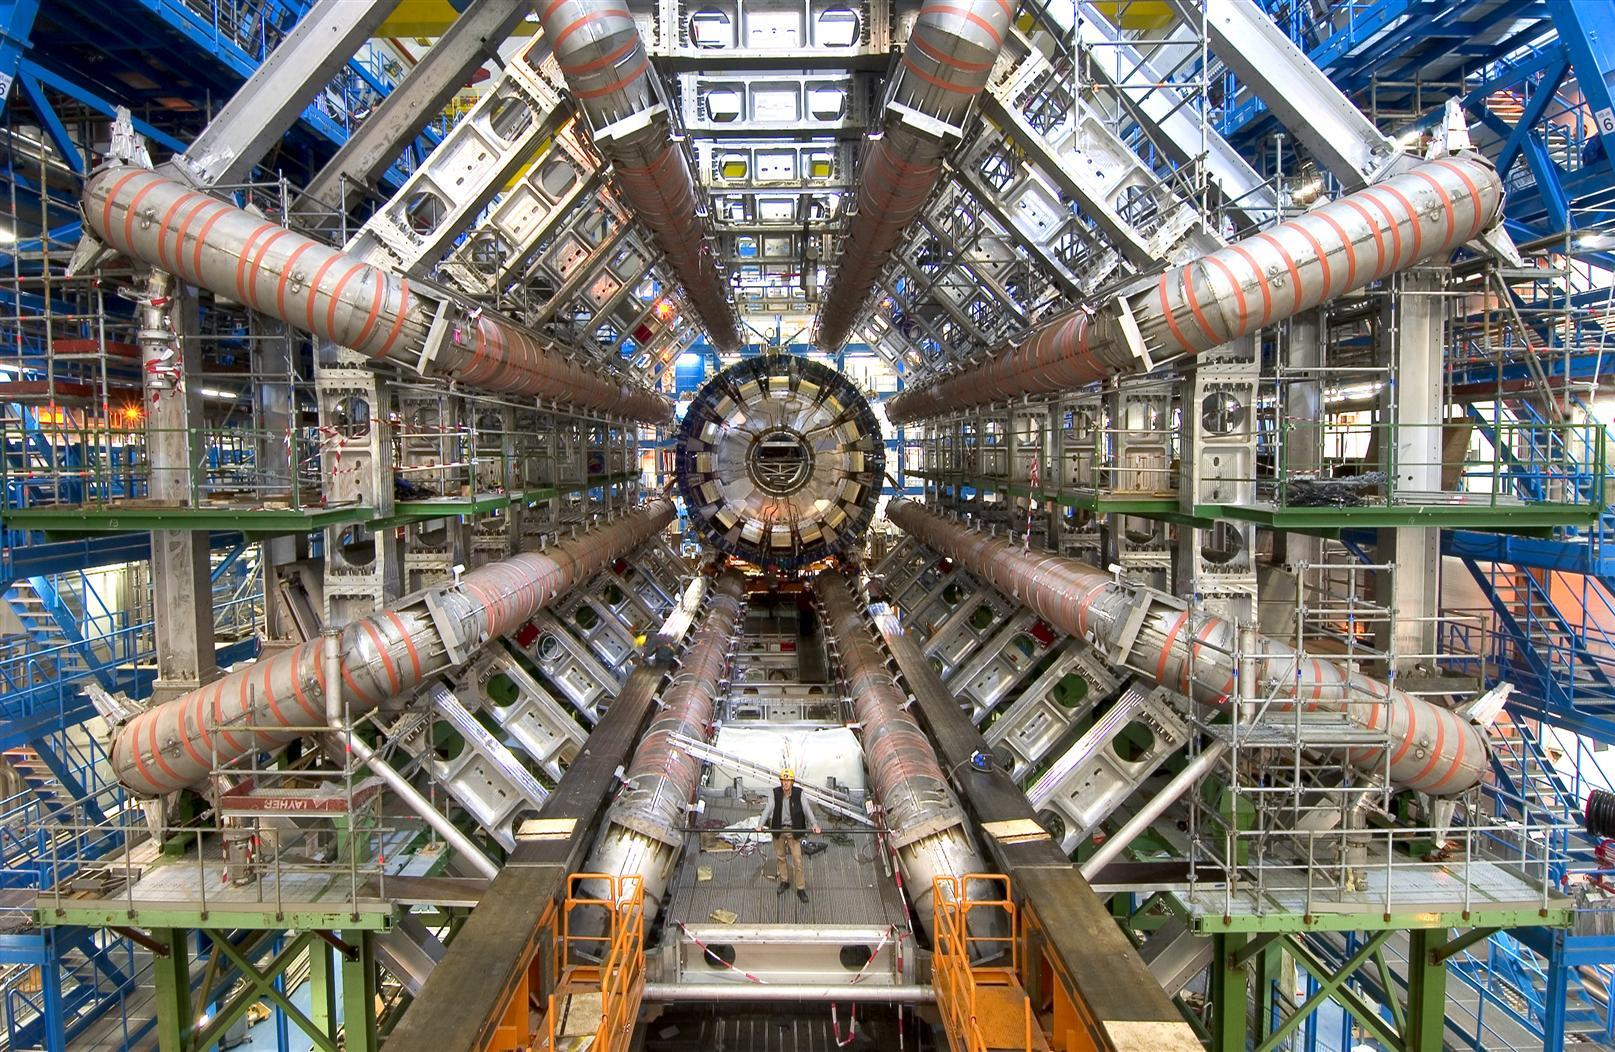
\includegraphics[width=7cm]{ATLASLHC.jpg}\hss}\hfill\null\newline
  	
 	Expériences CDF et D0 (Fermilab)
  	
  	 \textsc{\begin{figure}[h]
     \begin{minipage}[c]{.46\linewidth}
         \centering
         
\includegraphics[width=7cm]{CDFLOGO.png}
     \end{minipage}
     \hfill%
     \begin{minipage}[c]{.46\linewidth}
         \centering
         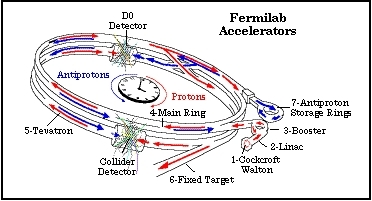
\includegraphics[width=7cm]{D0.jpg}
     \end{minipage}
 	\end{figure}}
  	
	R\&D en vue du Super LHC et pour un Futur collisionneur linéaire
	
	\hfill\hbox to 0pt{\hss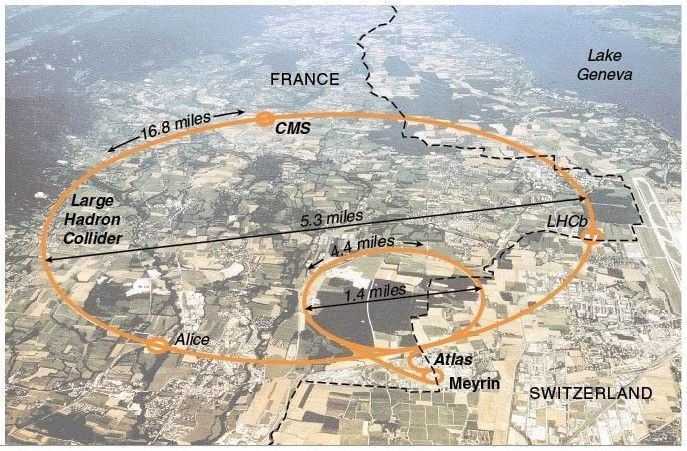
\includegraphics[width=7cm]{SLHC.jpg}\hss}\hfill\null\newline  	
  
  \item PHYSIQUE DES SAVEURS
  
  	Violation de symétrie CP : BaBar (Slac) et LHCb au LHC (Cern) 
  	Étude des neutrinos : T2K
  	PMPP (Phénoménologie et Modélisation en Physique des Particules)

  	\textsc{\begin{figure}[h]
     \begin{minipage}[c]{.46\linewidth}
         \centering
         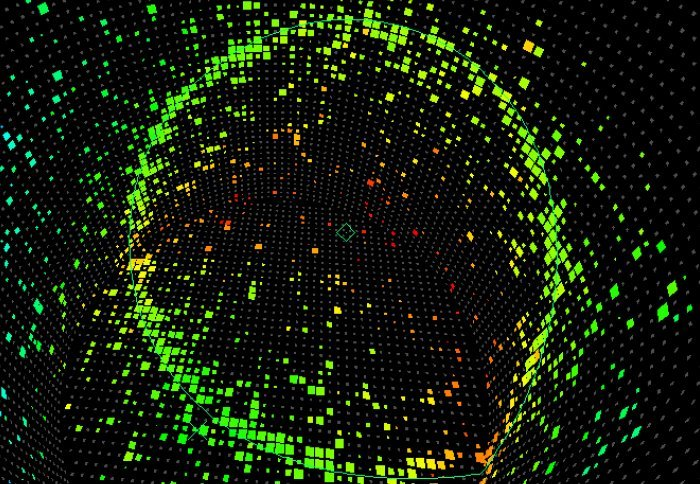
\includegraphics[width=7cm]{T2K.jpg}
     \end{minipage}
     \hfill%
     \begin{minipage}[c]{.46\linewidth}
         \centering
         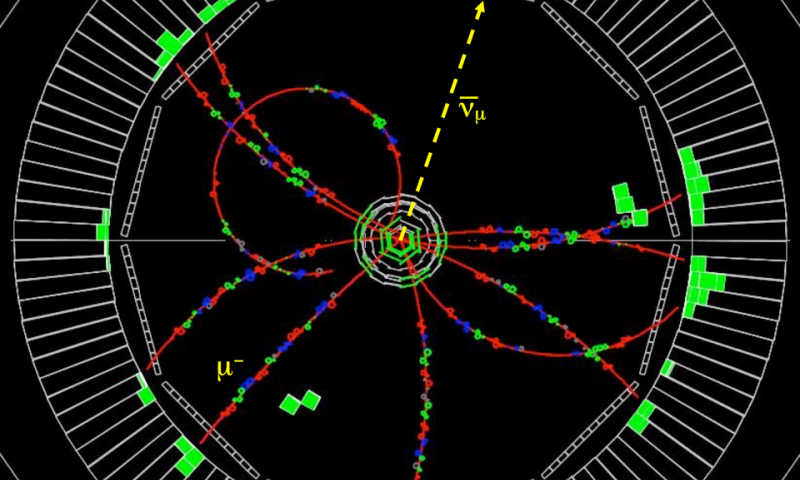
\includegraphics[width=7cm]{SLACBABAR.png}
     \end{minipage}
 	\end{figure}}
  	 
  \item ASTROPARTICULES Rayons cosmiques de hautes énergies
  
  	Photons de hautes énergies dans l’Univers : HESS, CTA
  	Étude des rayons cosmiques aux énergies extrêmes : Observatoire Auger
  	
  	\textsc{\begin{figure}[h]
     \begin{minipage}[c]{.46\linewidth}
         \centering
         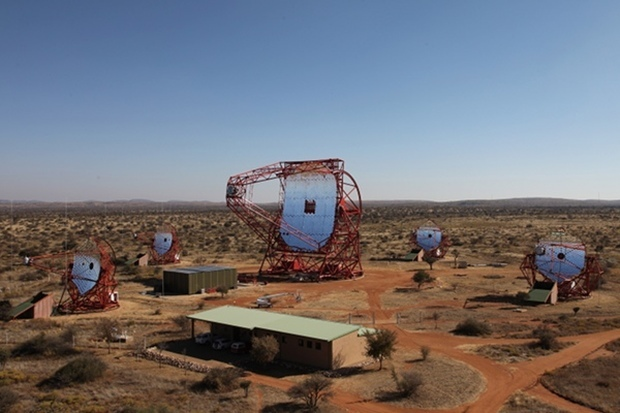
\includegraphics[width=7cm]{hesscta.jpg}
     \end{minipage}
     \hfill%
     \begin{minipage}[c]{.46\linewidth}
         \centering
         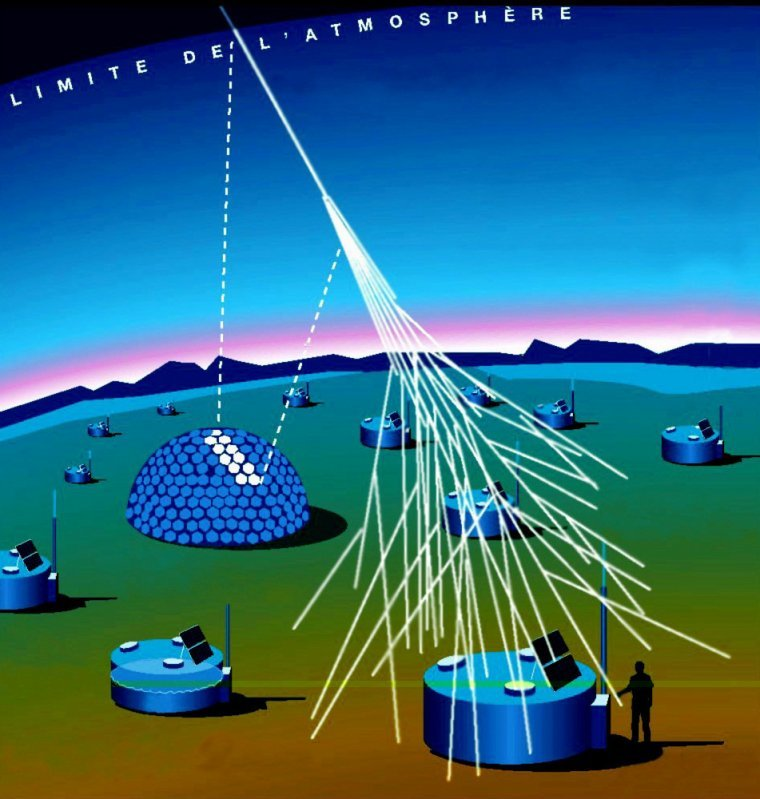
\includegraphics[width=7cm]{auger.jpg}
     \end{minipage}
 	\end{figure}}
 	\newpage
  
  \item Cosmologie
  
  	Supernovæ (SCP, SNF, SNLS) 
  	LSST
  	EUCLID
  	DSA  
  	
  	\hfill\hbox to 0pt{\hss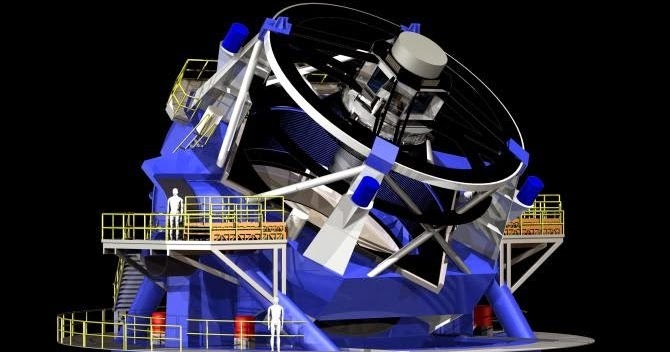
\includegraphics[width=7cm]{lsst.jpg}\hss}\hfill\null\newline
  	
  \end{itemize}
  
  
  \chapter{Présentation du projet "CHAMP"}
  
\part{Recherche Documentaire}

\part{Travaux menés}


\end{document}

%Mettre deux éléments l'un à coté de l'autre horizontalement
% \textsc{\begin{figure}[h]
%     \begin{minipage}[c]{.46\linewidth}
%         \centering
%         \includegraphics[width=7cm]{tp1_g1.png}
%     \end{minipage}
%     \hfill%
%     \begin{minipage}[c]{.46\linewidth}
%         \centering
%         \includegraphics[width=7cm]{tp1_g2.png}
%     \end{minipage}
% \end{figure}}